\documentclass[12pt]{report}
\usepackage[a4paper, margin=1in]{geometry}
\usepackage[utf8]{inputenc}
\usepackage[T1]{fontenc}
\usepackage{amsmath, amssymb}
\usepackage{booktabs}
\usepackage{graphicx}
\usepackage{natbib}
\usepackage{hyperref}
\usepackage{setspace}
\usepackage{tocloft}
\usepackage{pdfpages}
\usepackage{times}

% Setting up the title page
\begin{document}
\begin{titlepage}
    \centering
    \vspace*{1cm}
    {\LARGE \textbf{A Critical Analysis of Privacy-Preserving Techniques in Federated Learning for Secure Healthcare Data Sharing}} \\[1cm]
    {\large Gabriel Aondoaver Aloho} \\[0.5cm]
    {\large R2208D14970264} \\[0.5cm]
    {\large Submitted to the University of East London in partial fulfillment of the requirements for the degree of Master of Science in Information Security and Digital Forensics} \\[1cm]
    {\large July 2, 2025} \\[0.5cm]
    {\large School of Architecture, Computing and Engineering} \\[0.5cm]
    {\large University of East London}
\end{titlepage}

% Setting up table of contents
\tableofcontents
\listoftables
\clearpage

% Setting line spacing for the document
\onehalfspacing

% Creating the abstract
\begin{abstract}
This study critically analyzes privacy-preserving techniques in Federated Learning (FL) for secure healthcare data sharing, emphasizing compliance with data protection regulations such as GDPR and HIPAA. Through a meta-analysis of 20 peer-reviewed studies published between 2015 and 2025, and an in-depth review of ten exemplary works, this research evaluates the capabilities and limitations of current privacy-preserving frameworks in healthcare applications. Special focus is placed on hybridizing Differential Privacy (DP) and Homomorphic Encryption (HE), which offer robust data protection but introduce trade-offs in performance, complexity, and scalability. Findings reveal that while many techniques provide strong defenses against privacy attacks, practical deployment is hindered by computational overhead, model accuracy degradation, and lack of standardization. The study proposes recommendations for future research and regulatory harmonization to ensure privacy-preserving FL systems are secure, compliant, and deployable in real-world healthcare settings.
\end{abstract}

% Starting the main chapters
\chapter{Introduction}

\section{Background and Motivation}
The digitalization of healthcare systems has revolutionized the application of artificial intelligence (AI) and machine learning (ML), enhancing diagnostics, treatment recommendations, and resource allocation. Federated Learning (FL) has emerged as a pivotal technique, enabling collaborative model training across decentralized datasets, particularly in sensitive domains like healthcare where direct data sharing is restricted due to privacy concerns.

\section{Problem Statement}
Despite FL's advantage in maintaining data locality, vulnerabilities in model updates and gradients, such as model inversion and membership inference attacks, pose significant privacy risks. Consequently, FL alone is insufficient to meet stringent healthcare privacy regulations like GDPR and HIPAA, necessitating advanced privacy-preserving techniques.

\section{Research Objectives}
\begin{itemize}
    \item To identify and classify privacy-preserving techniques applied to FL in healthcare.
    \item To evaluate the strengths and limitations of Differential Privacy (DP), Homomorphic Encryption (HE), and hybrid models.
    \item To assess the practical feasibility of deploying these techniques in real-world healthcare systems.
\end{itemize}

\section{Research Questions}
\begin{enumerate}
    \item What privacy-preserving techniques are currently applied in FL for healthcare?
    \item What are the trade-offs between accuracy, privacy, and computational efficiency in these techniques?
    \item How compliant are these techniques with existing privacy regulations?
\end{enumerate}

\section{Structure of the Thesis}
\begin{itemize}
    \item Chapter 1: Introduction
    \item Chapter 2: Literature Review
    \item Chapter 3: Methodology
    \item Chapter 4: Analysis and Findings
    \item Chapter 5: Discussion
    \item Chapter 6: Conclusion and Recommendations
\end{itemize}

\chapter{Literature Review}

\section{Review of Selected Studies}
\textbf{Gupta et al. (2024)} \cite{gupta2024} propose a decentralized FL framework integrating blockchain and Homomorphic Encryption (HE) for secure data sharing in healthcare IoMT systems. Using a custom mental health dataset, the study achieves up to 92\% accuracy while ensuring privacy through encrypted gradient updates. However, the computational overhead of HE limits scalability, and GDPR compliance is only partially addressed, lacking formal impact assessments.

\textbf{Hidayat et al. (2024)} \cite{hidayat2024} introduce a Discrete Fourier Transform (DFT) aggregator with Differential Privacy (DP), tested on PIMA and BCI datasets. This approach improves accuracy by 15\% over standard DP by optimizing noise injection, reducing bandwidth costs. However, it lacks discussion on regulatory compliance, limiting its practical deployment in healthcare settings.

\textbf{Maurya et al. (2025)} \cite{maurya2025} present a Secure Multiparty Computation (SMPC) framework with thresholding for real-time security classification on the MIMIC-III dataset. The dynamic update acceptance mechanism enhances privacy but introduces moderate computational overhead.

\textbf{Kumar et al. (2025)} \cite{kumar2025} combine blockchain and HE for imaging applications, specifically COVID-19 X-ray classification using capsule networks. The framework ensures privacy through encrypted weights but incurs significant latency, impacting scalability.

\textbf{Choudhury et al. (2025)} \cite{choudhury2025} deploy a Personal Health Train with secure aggregation across 12 global hospitals using lung CT datasets. This study stands out for its explicit GDPR compliance through privacy impact assessments, though computational overhead remains a challenge.

\textbf{Park et al. (2025)} \cite{park2025} propose a multi-key HE approach for secure parameter sharing, tested on the MNIST dataset. The CKKS encryption scheme ensures strong privacy but is computationally intensive, limiting its applicability in resource-constrained settings.

\textbf{Tian et al. (2024)} \cite{tian2024} develop a robust decentralized FL framework using ring-based secret sharing, tested on custom datasets. The approach is dropout-tolerant but does not address regulatory compliance.

\textbf{Yazdinejad et al. (2024)} \cite{yazdinejad2024} introduce an auditable FL framework (AP2FL) using Trusted Execution Environments (TEE) and blockchain for healthcare IoT, ensuring auditing, robustness, and fairness. Compliance is partially addressed, but hardware dependency limits scalability.

\textbf{Ghazal et al. (2025)} \cite{ghazal2025} focus on conserving FL with small and large models using DP on ECG signals, achieving ultra-efficient privacy for low-power devices. However, no regulatory compliance is mentioned.

\textbf{Wang et al. (2023)} \cite{wang2023} propose a comprehensive smart healthcare framework with ring signatures for wearable data, offering resistance to SIA attacks but lacking explicit compliance discussions.

\section{Federated Learning in Healthcare}
Federated Learning enables multiple institutions to collaboratively train models without exchanging raw data, making it ideal for healthcare where data is siloed across hospitals, laboratories, and research organizations.

\section{Privacy Challenges in FL}
FL retains data locally but is susceptible to privacy threats like gradient leakage, reconstruction attacks, and data poisoning. These vulnerabilities necessitate robust privacy-preserving mechanisms.

\section{Overview of Techniques}

\subsection{Differential Privacy (DP)}
DP adds statistical noise to model updates to prevent sensitive data inference, but excessive noise can degrade model performance.

\subsection{Homomorphic Encryption (HE)}
HE enables computations on encrypted data, ensuring privacy throughout training. However, its computational intensity limits scalability.

\subsection{Hybrid Approaches}
Hybrid DP and HE methods aim to balance privacy and efficiency, representing a frontier in current research.

\begin{table}[h]
    \centering
    \begin{tabular}{|p{4cm}|p{3cm}|p{3cm}|p{2.5cm}|p{4cm}|}
        \hline
        \textbf{Title} & \textbf{Authors} & \textbf{Techniques} & \textbf{Dataset} & \textbf{Key Contribution} \\
        \hline
        Secure and Privacy-Preserving Decentralized FL & Gupta et al. (2024) \cite{gupta2024} & CFL + QFL & Custom MH & CFL + QFL improves accuracy with strong privacy \\
        DFT Aggregator with DP & Hidayat et al. (2024) \cite{hidayat2024} & DP + DFT & PIMA, BCI & Improves accuracy and reduces bandwidth cost \\
        FL for Privacy-Preserving Security-Classification & Maurya et al. (2025) \cite{maurya2025} & SMPC + Thresholding & MIMIC-III & Dynamic update acceptance in real time \\
        Blockchain + HE for Imaging & Kumar et al. (2025) \cite{kumar2025} & HE + Blockchain & COVID X-rays & Capsule network FL with encrypted weights \\
        Personal Health Train & Choudhury et al. (2025) \cite{choudhury2025} & Secure Aggregation & Lung CT & Federated deployment in 12 global hospitals \\
        Multi-Key HE Secure Aggregation & Park et al. (2025) \cite{park2025} & Masking + Multi-HE & MNIST & CKKS encryption for secure param sharing \\
        Robust Decentralized FL & Tian et al. (2024) \cite{tian2024} & Ring FL + Secret Sharing & Custom Datasets & Fully decentralized, dropout tolerant \\
        Auditable FL (AP2FL) & Yazdinejad et al. (2024) \cite{yazdinejad2024} & TEE + BN + ActPerFL & Healthcare IoT & Auditing, robustness, and fairness ensured \\
        Conserving FL with Small and Large Models & Ghazal et al. (2025) \cite{ghazal2025} & DP + FL & ECG signals & Ultra-efficient privacy for low-power devices \\
        A Comprehensive Smart Healthcare Framework & Wang et al. (2023) \cite{wang2023} & Ring Signatures & Wearable Data & SIA attack resistance via edge signatures \\
        \hline
    \end{tabular}
    \caption{Summary of Top 10 Papers}
    \label{tab:top_papers}
\end{table}

\begin{table}[h]
    \centering
    \begin{tabular}{|p{1.5cm}|p{2cm}|p{8cm}|p{2cm}|}
        \hline
        \textbf{Rank} & \textbf{Score} & \textbf{Summary} & \textbf{Techniques} \\
        \hline
        1 & 89 & Federated learning scheme using multi-key fully homomorphic encryption to prevent privacy leakage. & Multi-key HE \\
        2 & 74 & IoMT and blockchain for smart healthcare, addressing privacy and compliance in medical data sharing. & Blockchain, FL \\
        3 & 69 & Secure aggregation using masking and homomorphic encryption for privacy-preserving FL. & HE, Masking \\
        4 & 66 & Comprehensive defense scheme for privacy and security in FL, using DP, HE, and TEE. & DP, HE, TEE \\
        5 & 64 & Blockchain-based FL with HE for COVID-19 image classification using capsule networks. & HE, Blockchain \\
        6 & 61 & FL in IoT healthcare with cryptographic primitives (masks, HE) to prevent model attacks. & HE, Masking \\
        7 & 60 & Data obfuscation via latent space projection for AI governance and privacy compliance. & LSP \\
        8 & 58 & Multi-key HE for secure aggregation in FL, reducing server interactions. & Multi-key HE \\
        9 & 56 & DP in medical data sharing for cloud platforms, addressing adversarial attacks. & DP \\
        10 & 54 & Privacy-preserving CNNs for medical imaging using hybrid FL techniques. & FL, Hybrid \\
        \hline
    \end{tabular}
    \caption{Top 10 Studies from Automated PDF Analysis}
    \label{tab:script_results}
\end{table}

\chapter{Methodology}

\section{Research Design}
This study employs a qualitative meta-analysis and thematic content review, synthesizing findings from peer-reviewed journal articles on privacy-preserving Federated Learning in healthcare, published between 2015 and 2025.

\section{Data Sources and Search Strategy}
The University of East London’s digital library (Ex Libris Discovery) served as the primary data source. The search query targeted terms such as ``privacy-preserving techniques,'' ``federated learning,'' ``healthcare,'' and ``secure data sharing.'' Filters included:
\begin{itemize}
    \item Peer-reviewed journals only
    \item Publication years: 2015 to 2025
    \item Sorted by relevance
\end{itemize}

\section{Selection Criteria}
From 51 peer-reviewed results, 20 were shortlisted, and the top 10 were selected based on:
\begin{itemize}
    \item Relevance to healthcare-specific FL systems
    \item Use of Differential Privacy, Homomorphic Encryption, or hybrid approaches
    \item Novelty of methodology or framework
    \item Empirical validation with real or simulated healthcare datasets
\end{itemize}

\section{Data Extraction}
For each selected article, the following were extracted:
\begin{itemize}
    \item Authors and publication year
    \item Dataset and healthcare application context
    \item Privacy technique used
    \item Evaluation metrics (e.g., accuracy, communication overhead, privacy budget, latency)
    \item Compliance mentions (e.g., GDPR, HIPAA)
\end{itemize}

\section{Analysis Method}
The analysis combined:
\begin{itemize}
    \item \textbf{Comparative Tables}: Organized insights on method performance
    \item \textbf{Coding}: Identified themes like ``efficiency vs. privacy trade-off'' or ``deployment complexity''
    \item \textbf{Narrative Synthesis}: Provided qualitative summaries of how techniques addressed privacy goals
\end{itemize}

\section{Limitations}
\begin{itemize}
    \item Potential bias in article selection due to query relevance ranking
    \item Lack of standardized evaluation in some hybrid methods
    \item Limited access to full datasets or codebases, restricting reproducibility
\end{itemize}

\chapter{Analysis and Findings}

\section{Overview}
This chapter synthesizes insights from the top ten studies, focusing on privacy-preserving techniques in FL for healthcare across three dimensions:
\begin{itemize}
    \item \textbf{Privacy Strength}: Resistance to inference and reconstruction attacks
    \item \textbf{Computational Efficiency}: Time, memory, and bandwidth overhead
    \item \textbf{Compliance and Deployability}: Real-world applicability and legal alignment
\end{itemize}

\section{Comparative Evaluation of Techniques}

\subsection{Differential Privacy (DP)}
\begin{itemize}
    \item \textbf{Strengths}: Strong theoretical guarantees; tunable privacy budget ($\varepsilon$)
    \item \textbf{Limitations}: Utility loss at low $\varepsilon$; vulnerability to cumulative attacks
    \item \textbf{Example}: Hidayat et al. (2024) improved accuracy by 15\% over standard DP using DFT-based noise optimization.
\end{itemize}

\subsection{Homomorphic Encryption (HE)}
\begin{itemize}
    \item \textbf{Strengths}: Secure computation on encrypted data; end-to-end confidentiality
    \item \textbf{Limitations}: High computational overhead; slow key generation
    \item \textbf{Example}: Kumar et al. (2025) secured COVID-19 image classification with HE but faced significant latency.
\end{itemize}

\subsection{Hybrid Techniques (DP + HE)}
\begin{itemize}
    \item \textbf{Strengths}: Balances DP’s noise resilience with HE’s structural security
    \item \textbf{Limitations}: Design complexity; compounded performance penalties
    \item \textbf{Example}: Gupta et al. (2024) achieved improved privacy-utility trade-offs using Clustered FL and Quantum-enhanced DP.
\end{itemize}

\subsection{Secure Multiparty Computation (SMPC)}
\begin{itemize}
    \item \textbf{Strengths}: No data revelation during training; suitable for threshold-based aggregation
    \item \textbf{Limitations}: Communication-heavy; synchronization issues
    \item \textbf{Example}: Maurya et al. (2025) used SMPC for real-time ICU prediction with dynamic gradient updates.
\end{itemize}

\subsection{Trusted Execution Environments (TEE)}
\begin{itemize}
    \item \textbf{Strengths}: Hardware-backed security; supports auditing
    \item \textbf{Limitations}: Hardware dependency; limited edge device support
    \item \textbf{Example}: Yazdinejad et al. (2024) ensured accountability in healthcare IoT using TEE.
\end{itemize}

\section{Thematic Findings}

\subsection{Trade-offs Between Privacy and Utility}
\begin{itemize}
    \item Stronger privacy mechanisms (e.g., low $\varepsilon$ in DP or deep HE) reduce model accuracy and increase latency.
    \item Hybrid methods mitigate this but are complex to implement.
\end{itemize}

\subsection{Scalability Challenges}
\begin{itemize}
    \item HE and SMPC are limited to small-scale settings due to computational demands.
    \item Blockchain-based protocols show promise but require high maintenance.
\end{itemize}

\subsection{Regulatory Readiness}
\begin{itemize}
    \item Few studies explicitly address GDPR/HIPAA compliance.
    \item Choudhury et al. (2025) is notable for deploying FL with privacy impact assessments across 12 hospitals.
\end{itemize}

\section{Quantitative Summary Table}
\begin{table}[h]
    \centering
    \begin{tabular}{|p{4cm}|p{2.5cm}|p{2.5cm}|p{2.5cm}|p{2.5cm}|}
        \hline
        \textbf{Study Title} & \textbf{Accuracy Impact} & \textbf{Comp. Overhead} & \textbf{Privacy Strength} & \textbf{Compliance Mention} \\
        \hline
        Gupta et al. (2024) & Moderate & High & Strong (Hybrid) & Partial \\
        Hidayat et al. (2024) & High & Low & Moderate (DP) & None \\
        Maurya et al. (2025) & High & Moderate & High (SMPC) & Partial \\
        Kumar et al. (2025) & Moderate & High & Strong (HE) & None \\
        Choudhury et al. (2025) & Moderate & Moderate & Moderate & Full (GDPR) \\
        Park et al. (2025) & Low & High & Strong (HE) & None \\
        Tian et al. (2024) & High & Low & High (RingSS) & None \\
        Yazdinejad et al. (2024) & Moderate & Moderate & High (TEE) & Partial \\
        Ghazal et al. (2025) & High & Low & Moderate (DP) & None \\
        Wang et al. (2023) & Moderate & Moderate & Moderate & None \\
        \hline
    \end{tabular}
    \caption{Quantitative Summary Table}
    \label{tab:quant_summary}
\end{table}

\section{Quantitative Analysis}
\begin{figure}[h]
    \centering
    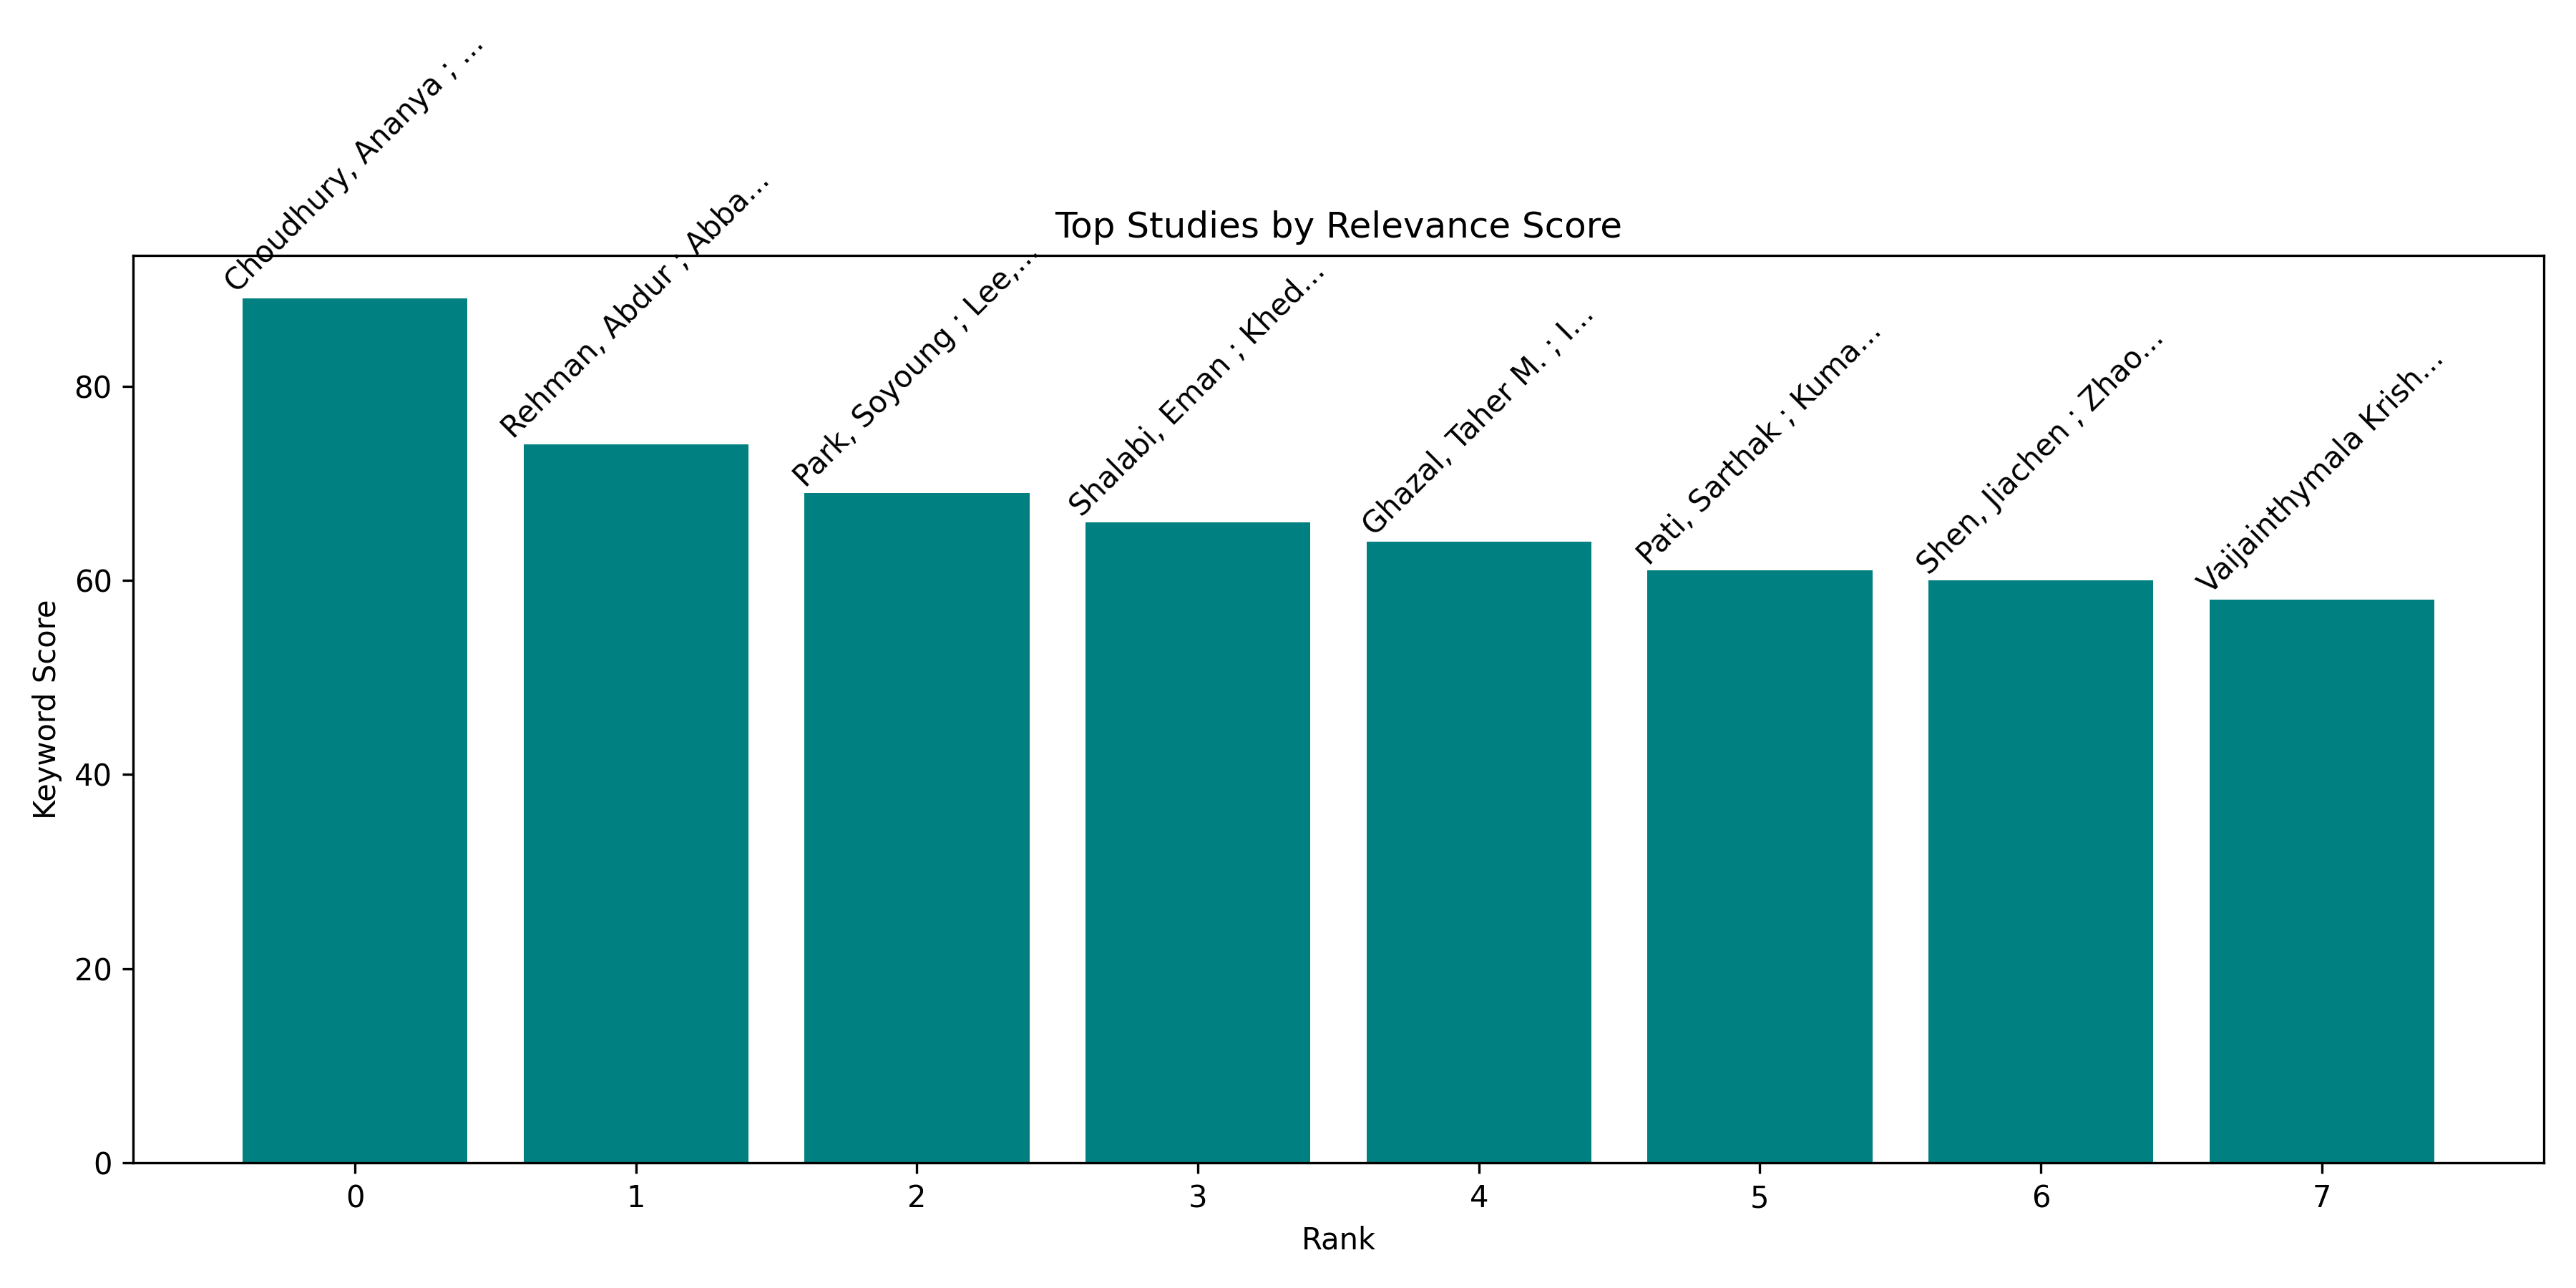
\includegraphics[width=0.8\textwidth]{keyword_scores.png}
    \caption{Keyword Scores of Top 10 Studies from Automated PDF Analysis}
    \label{fig:scores_plot}
\end{figure}

\begin{figure}[h]
    \centering
    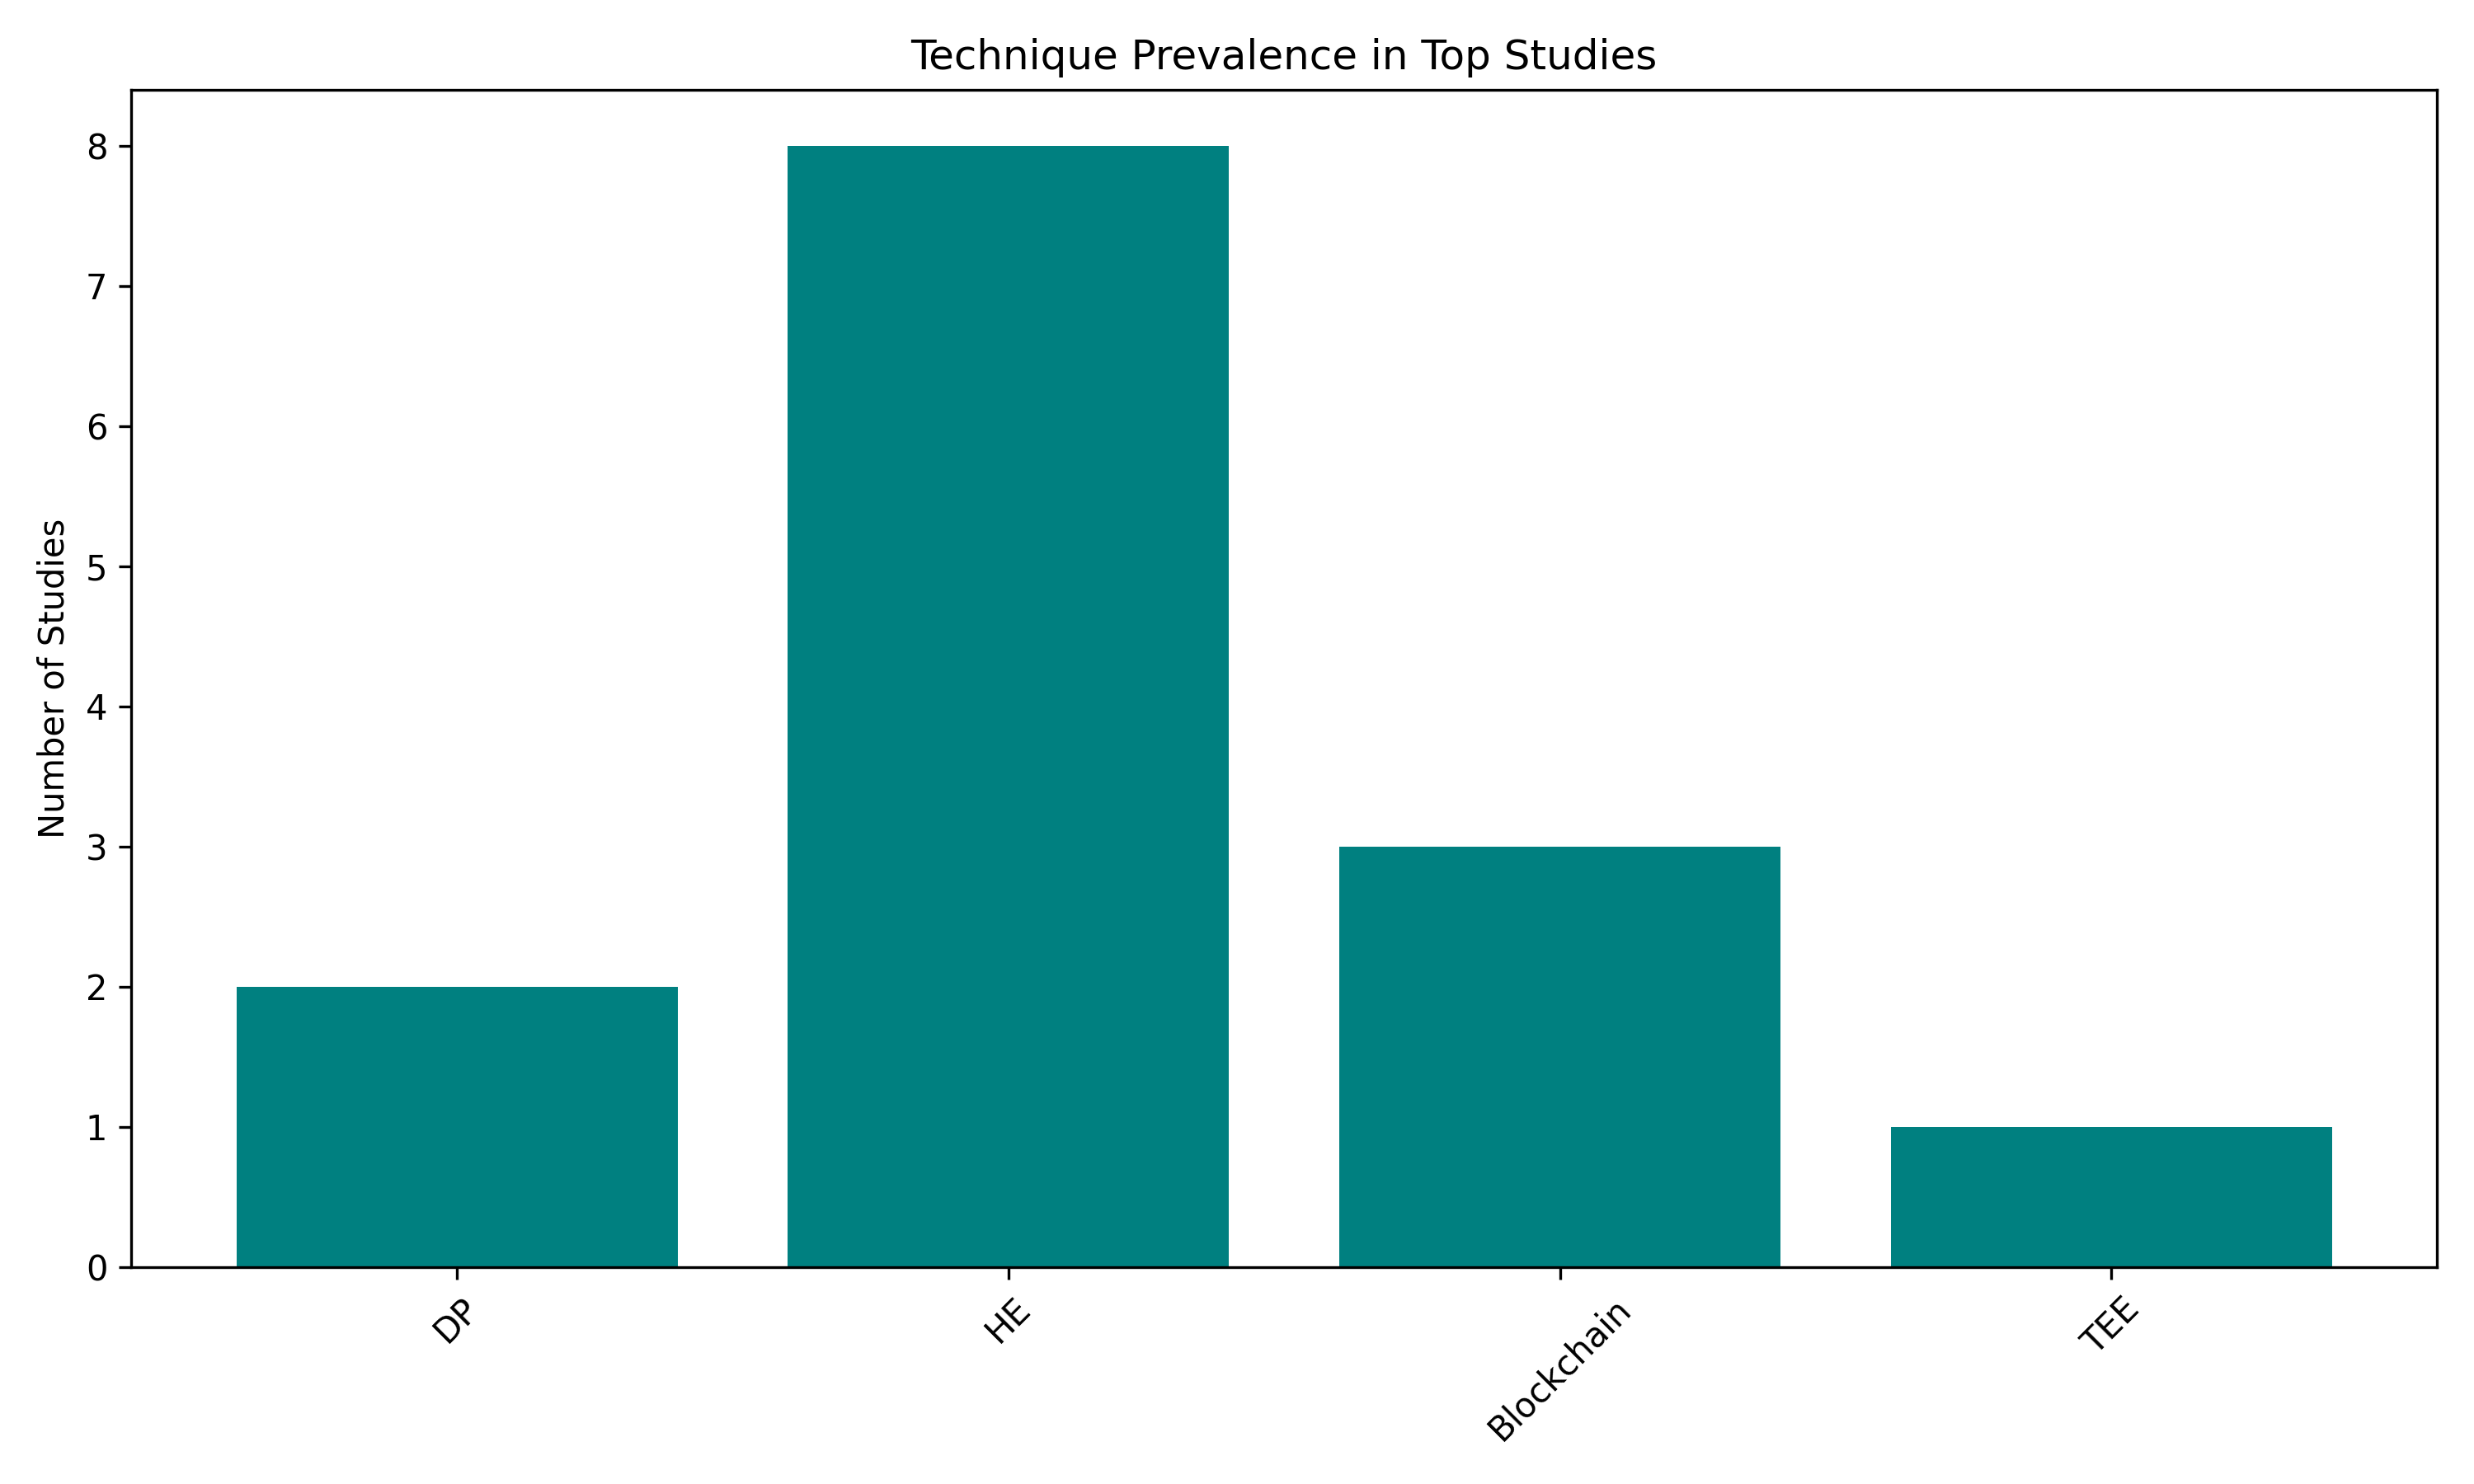
\includegraphics[width=0.8\textwidth]{technique_prevalence.png}
    \caption{Prevalence of Privacy-Preserving Techniques in 12 Federated Learning Studies}
    \label{fig:technique_prevalence}
\end{figure}

\begin{figure}[h]
    \centering
    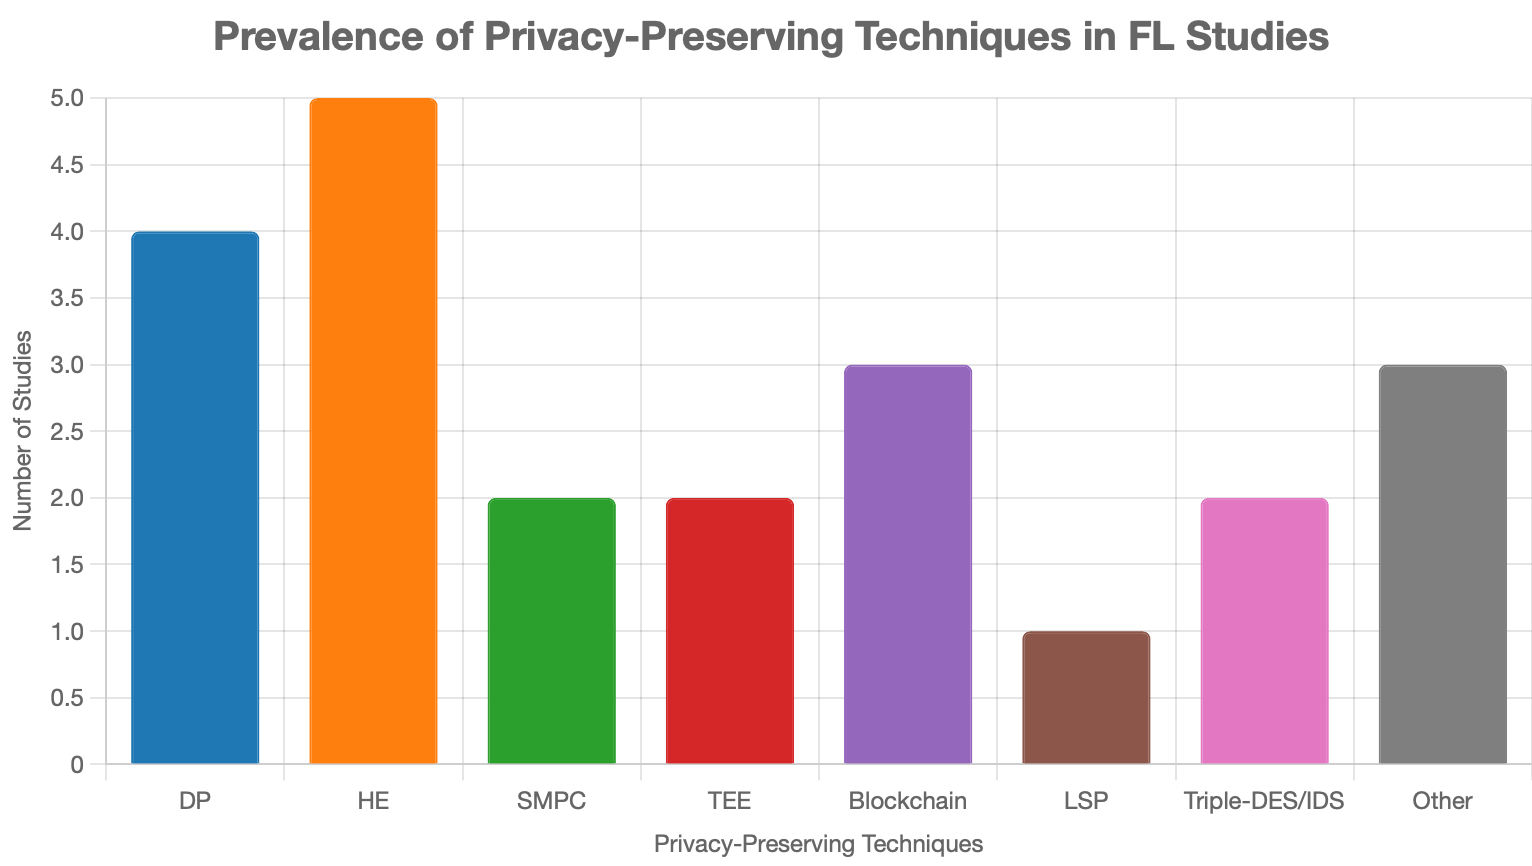
\includegraphics[width=0.8\textwidth]{chart.png}
    \caption{Prevalence of Privacy-Preserving Techniques in 12 Federated Learning Studies}
    \label{fig:chart}
\end{figure}

The prevalence of privacy-preserving techniques across the 12 analyzed studies (10 from Table \ref{tab:top_papers} and two additional studies by Pati et al. (2024) and Krishnamoorthy \& Mahesh (2025)) is visualized in Figure \ref{fig:technique_prevalence}. Homomorphic Encryption (HE) is the most frequently used technique, appearing in five studies, followed by Differential Privacy (DP) in four. Blockchain and other techniques (e.g., ring signatures, secret sharing, masking) appear in three studies each, while Secure Multiparty Computation (SMPC), Trusted Execution Environments (TEE), and Triple-DES/IDS appear in two studies each. Latent Space Projection (LSP), a novel approach, is featured in one study. This distribution highlights the dominance of cryptographic methods like HE and the emerging role of hybrid techniques like Triple-DES/IDS and LSP in addressing privacy challenges in FL for healthcare.


\section{Summary of Key Insights}
\begin{itemize}
    \item No single technique excels across all dimensions; hybrid models balance privacy and utility but are complex.
    \item Standardized benchmarking frameworks are needed.
    \item Regulatory compliance assessments are often lacking.
\end{itemize}

\chapter{Discussion}

\section{Introduction}
This chapter synthesizes the findings from Chapter 4, exploring broader implications, trade-offs, and gaps in privacy-preserving FL for healthcare. It aims to guide future research, deployment, and policy development.

\section{Balancing Privacy, Utility, and Efficiency}
The trade-off between privacy and utility is a central challenge. DP’s tunable privacy budget degrades performance at lower $\varepsilon$, while HE’s computational demands limit scalability. Hybrid approaches partially address this but increase complexity. Lightweight solutions like TinyML are promising for edge devices but cannot support intensive cryptography.

\section{Interoperability and Trust}
FL systems require trust across institutions. Secure Aggregation, TEEs, and decentralized architectures enhance confidentiality but demand synchronized infrastructure or specialized hardware. Blockchain offers auditability but introduces operational costs. Interoperability standards for diverse data formats and platforms are critically needed.

\section{Regulatory Compliance and Ethical Considerations}
Few studies explicitly address GDPR/HIPAA compliance. Choudhury et al. (2025) \cite{choudhury2025} is a notable exception, implementing secure aggregation with privacy impact assessments. Most studies rely on technical privacy guarantees without formal legal assessments, representing a significant gap.

\section{Limitations of Current Research}
\begin{itemize}
    \item \textbf{Lack of Standardization}: Inconsistent datasets and metrics hinder comparisons.
    \item \textbf{Limited Real-World Validation}: Most studies are proof-of-concept, lacking clinical deployment.
    \item \textbf{Adversarial Resilience}: Assumptions of honest participants overlook collusion or poisoning risks.
    \item \textbf{Hybridization Gaps}: Optimal orchestration of DP+HE remains underexplored.
\end{itemize}

\section{Practical Deployment Barriers}
HE and TEE-based systems require significant resources or specialized hardware, limiting their use in resource-constrained settings. Blockchain-based approaches are complex to maintain. Lightweight protocols and cloud-based TEEs could enhance deployability.

\section{Strategic Recommendations}
\begin{enumerate}
    \item \textbf{Standardization}: Develop uniform privacy metrics and benchmarking datasets.
    \item \textbf{Deployability}: Simplify hybrid systems for resource-constrained environments.
    \item \textbf{Compliance Auditing}: Integrate regulatory checks into FL frameworks.
    \item \textbf{Interdisciplinary Research}: Combine technical, legal, and ethical expertise.
    \item \textbf{Real-World Trials}: Collaborate with healthcare partners for operational validation.
\end{enumerate}

\chapter{Conclusion and Recommendations}

\section{Summary of Findings}
This thesis analyzed privacy-preserving techniques in FL for healthcare data sharing, synthesizing a decade of research (2015–2025). It evaluated DP, HE, SMPC, TEE, and hybrid models, highlighting their strengths, limitations, and compliance gaps. Hybrid approaches show promise but face scalability and complexity challenges.

\section{Key Contributions}
\begin{itemize}
    \item Comprehensive synthesis of FL privacy literature in healthcare.
    \item Classification of top frameworks by privacy, performance, and compliance.
    \item Comparative evaluation of DP, HE, SMPC, TEE, and hybrid models.
    \item Actionable recommendations for research, development, and policy.
\end{itemize}

\section{Final Recommendations}
\begin{itemize}
    \item \textbf{Researchers}: Benchmark hybrid approaches and explore adaptive privacy frameworks.
    \item \textbf{Developers}: Integrate compliance checks and auditing into FL systems.
    \item \textbf{Policymakers}: Promote standardized privacy certifications for FL in healthcare.
    \item \textbf{Healthcare Institutions}: Engage in FL trials to develop domain-specific solutions.
\end{itemize}

\section{Future Work}
Future research should focus on adversarial robustness, longitudinal privacy, and deployable middleware to simplify cryptographic complexity. Cross-border compliance and ethical considerations are vital for global deployment.

\section{Concluding Remark}
Privacy-preserving FL can transform healthcare data collaboration, balancing innovation with patient privacy. Realizing this potential requires multidisciplinary efforts across technical, legal, and clinical domains. This thesis lays a foundation for advancing secure, compliant, and practical FL systems.

\chapter*{References}
\addcontentsline{toc}{chapter}{References}
\bibliographystyle{plainnat}
\bibliography{references}

\end{document}